\documentclass[11pt]{standalone}
\usepackage{amssymb}
\usepackage{amsmath}
\usepackage[no-math]{fontspec}
\usepackage{unicode-math}
\usepackage{libertinus}
\usepackage{pgf,xcolor}
\usepackage{tikz}
\usetikzlibrary{arrows.meta, backgrounds, calc}
\usepackage{pgfplots}
\pgfplotsset{compat=newest}

\definecolor{my_darkgray}{HTML}{484949}
\definecolor{my_lightgray}{HTML}{F3F4F4}
\definecolor{my_darkblue}{HTML}{005A94}
\definecolor{my_lightblue}{HTML}{CCDEE9}
\definecolor{my_yellow}{HTML}{FFEC7F}
\definecolor{my_red}{HTML}{E60000}
\definecolor{my_orange}{HTML}{E87846}

\begin{document}
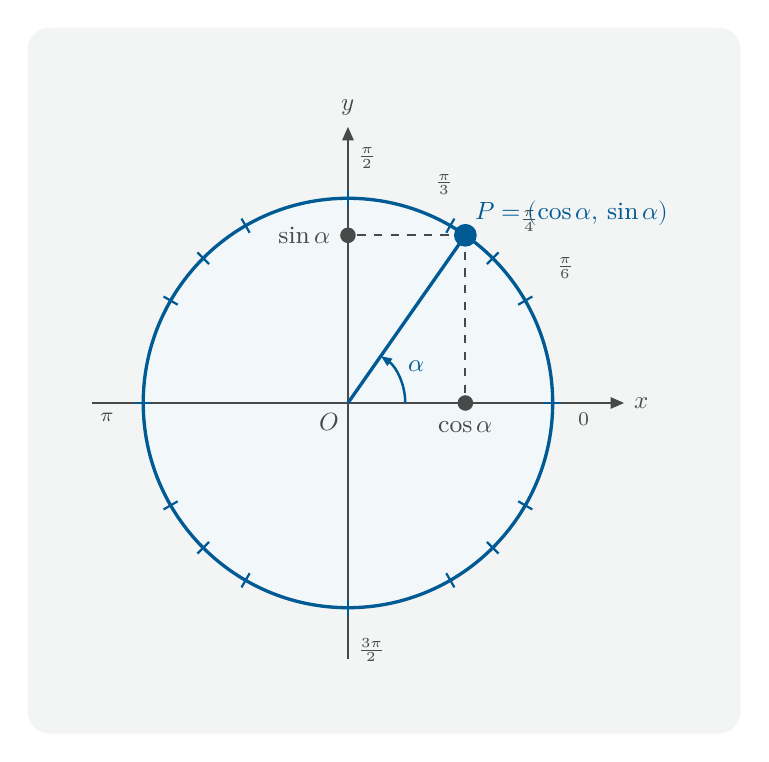
\begin{tikzpicture}[
    show background rectangle,
    background rectangle/.style={fill=my_lightgray, rounded corners=8pt},
    inner frame sep=0.8cm,
    scale=2.6,  % radius = 1 drawing unit -> visually ~2.6cm
]

% ── Coordinate definitions ───────────────────────────────────────────────────
% Generic angle alpha for the labeled point P
\pgfmathsetmacro{\anglealpha}{55}
\pgfmathsetmacro{\px}{cos(\anglealpha)}  % cos(55°) ≈ 0.574
\pgfmathsetmacro{\py}{sin(\anglealpha)}  % sin(55°) ≈ 0.819

% ── Unit circle ──────────────────────────────────────────────────────────────
\draw[my_lightblue, fill=my_lightblue!25, line width=0.6pt]
    (0,0) circle (1);
\draw[my_darkblue, line width=1.2pt] (0,0) circle (1);

% ── Coordinate axes ──────────────────────────────────────────────────────────
\draw[-{Triangle[length=5pt,width=4pt]}, my_darkgray, line width=1pt]
    (-1.25,0) -- (1.35,0) node[right, font=\small] {$x$};
\draw[-{Triangle[length=5pt,width=4pt]}, my_darkgray, line width=1pt]
    (0,-1.25) -- (0,1.35) node[above, font=\small] {$y$};

% ── Standard angle tick marks ─────────────────────────────────────────────────
% Mark ticks at all multiples of 30° and 45° on the circle.
\foreach \ang in {0,30,45,60,90,120,135,150,180,210,225,240,270,300,315,330} {
    \draw[my_darkblue, line width=0.8pt]
        ({0.96*cos(\ang)},{0.96*sin(\ang)}) --
        ({1.04*cos(\ang)},{1.04*sin(\ang)});
}

% ── Labels for key standard angles (first quadrant + axes) ───────────────────
% On-circle labels: place just outside the circle.
% Axis intercepts
\node[below right, font=\scriptsize, my_darkgray] at (1.08, 0)    {$0$};
\node[above right, font=\scriptsize, my_darkgray] at (0,    1.10) {$\frac{\pi}{2}$};
\node[below left,  font=\scriptsize, my_darkgray] at (-1.10,0)    {$\pi$};
\node[below right, font=\scriptsize, my_darkgray] at (0,   -1.10) {$\frac{3\pi}{2}$};

% First-quadrant standard angles
\node[above right, font=\scriptsize, my_darkgray]
    at ({1.12*cos(30)}, {1.12*sin(30)}) {$\frac{\pi}{6}$};
\node[above right, font=\scriptsize, my_darkgray]
    at ({1.12*cos(45)}, {1.12*sin(45)}) {$\frac{\pi}{4}$};
\node[above left,  font=\scriptsize, my_darkgray]
    at ({1.12*cos(60)}, {1.12*sin(60)}) {$\frac{\pi}{3}$};

% ── Radius line to point P ────────────────────────────────────────────────────
\draw[my_darkblue, line width=1.2pt] (0,0) -- (\px, \py);

% ── Dashed projections to the axes ───────────────────────────────────────────
% Vertical dashed line from P down to x-axis
\draw[dashed, my_darkgray, line width=0.7pt] (\px, \py) -- (\px, 0);
% Horizontal dashed line from P left to y-axis
\draw[dashed, my_darkgray, line width=0.7pt] (\px, \py) -- (0, \py);

% ── Point P on the circle ─────────────────────────────────────────────────────
\filldraw[my_darkblue] (\px, \py) circle (1.5pt);
\node[above right, font=\small, my_darkblue]
    at (\px, \py) {$P=(\cos\alpha,\,\sin\alpha)$};

% ── Foot of perpendicular on x-axis: marks cos(alpha) ───────────────────────
\filldraw[my_darkgray] (\px, 0) circle (1pt);
\node[below, font=\small, my_darkgray] at (\px, -0.04) {$\cos\alpha$};

% ── Foot of perpendicular on y-axis: marks sin(alpha) ───────────────────────
\filldraw[my_darkgray] (0, \py) circle (1pt);
\node[left, font=\small, my_darkgray] at (-0.04, \py) {$\sin\alpha$};

% ── Arc showing the angle alpha from the positive x-axis ─────────────────────
\draw[my_darkblue, line width=0.9pt, -{Triangle[length=4pt,width=3pt]}]
    (0.28, 0) arc[start angle=0, end angle=\anglealpha, radius=0.28];
\node[my_darkblue, font=\small] at ({0.38*cos(28)}, {0.38*sin(28)}) {$\alpha$};

% ── Origin label ─────────────────────────────────────────────────────────────
\node[below left, font=\small, my_darkgray] at (0,0) {$O$};

\end{tikzpicture}
\end{document}
